 %%%%%%%%%%%%%%%---SYNOPSIS--%%%%%%%%%%%%%%%%%%%%%%%%%%%

%%%%%%%%%%%%%%%%%%%%%%%%%%%%%%%%%%%%%%%%%%%%%%%%%%%%%%
\documentclass[12pt,a4paper,oneside]{report}
%\documentclass[12pt,a4paper,twoside]{book}

% -----------------------------
% Font fixes for pdfTeX + microtype
% -----------------------------
\usepackage[T1]{fontenc}
\usepackage{lmodern}

\usepackage{chngcntr}
%\counterwithin{figure}{chapter}
%\usepackage[nottoc]{tocbibind}
\usepackage{changepage}
\pagestyle{plain}
\usepackage{makeidx}
\usepackage{nomencl}
\usepackage{titlesec}
\usepackage{epsf}
\usepackage{graphicx}
\usepackage{amsmath}
\usepackage{amsfonts}
\usepackage{epstopdf}
\usepackage{comment}
\usepackage[hidelinks]{hyperref}
\hypersetup{
  hypertexnames=false,
  pdftitle={MS0240 CA3 Wages 2021 June Regression Report},
  pdfauthor={Goh Kun Ming},
  pdfsubject={Mathematics for Artificial Intelligence CA3},
  pdfkeywords={MS0240, regression, gradient descent, Singapore Polytechnic}
}
\setcounter{secnumdepth}{3}
\setcounter{tocdepth}{3}
\usepackage{fancyhdr}
\usepackage[english]{babel}
\usepackage{blindtext}
\usepackage{upquote}
\usepackage{fvextra}
\RecustomVerbatimEnvironment{verbatim}{Verbatim}{
  breaklines=true,
  breakanywhere=true,
  fontsize=\small
}
%\usepackage[titletoc]{appendix}
\usepackage{enumerate}
\usepackage{lipsum}

\usepackage[a4paper, inner=1.5cm, outer=3cm, top=2cm,bottom=3cm, bindingoffset=1cm]{geometry}
\textheight=235mm
\textwidth=145mm
\topmargin=0mm
\headheight=0mm
\headsep=0mm
\oddsidemargin=15mm
\evensidemargin=15mm

\makeindex
% \makeglossary removed: it is undefined unless a glossary package is loaded.

\graphicspath{{./figures/}{./assets/}}
\usepackage{float}

\usepackage[]{setspace}
\singlespacing

\usepackage{amssymb}
\setstretch{1}

\usepackage{cite}
\linespread{1.3}

\renewcommand{\thesection}{\arabic{section}}
\renewcommand{\thefigure}{\arabic{figure}}
\renewcommand{\thetable}{\arabic{table}}
\renewcommand{\theHfigure}{\arabic{figure}}
\renewcommand{\theHtable}{\arabic{table}}

\addto{\captionsenglish}{%
  \renewcommand{\bibname}{\LARGE References}
}

%***********************************************************

\begin{document}
\newgeometry{top=1in,bottom=1in,right=1in,left=1in}
\thispagestyle{empty}
\begin{center}
   {\Large\bf{MS0240 Mathematics for AI CA3 Report} \\}

			    
			       \vspace{0.3in}
			     
			      
  {\textbf{\textit{Wages 2021 June Regression Analysis\\}}}
		       
			     \vspace{0.4in}
			    {\large \bf Goh Kun Ming \\
			    P2415691\\
			    Diploma in Applied AI \& Analytics\\
			    AY2025/2026, Year 2 Semester 2}
			 
			  \vspace{0.3 in}

		       {\bf\textit{Submitted for the partial fulfilment of}}
		       
		       \vspace{0.3 in}

			    {\Large{\bf Mathematics for Artificial Intelligence \\ MS0240}\\}
                   \vspace{0.3in}
                {\bf\textit{Lecturer\\ }}
			{\Large{\bf Adj. Lect. Tan Lian Kuan}\\}		    
                \vspace{0.3in}
	      
\includegraphics[width=0.50\linewidth]{sp_logo.png}


			   \vspace{0.3in}
		     {\large\bf School of Computing\\}
   
			 {\large\bf  Singapore Polytechnic \\}
			     {\large\bf 500 Dover Rd, Singapore \\}
			     {\large\bf  2026 }
\end{center}
\date{}
\setcounter{page}{0}
\newpage
%****************************************************************


%====================================================================
\setcounter{page}{1}
%====================================================================
\section{Simple Linear Regression without Intercept}
\subsection{Model Definition}
In Model 1, we assume that the regression line passes through the origin.
The model is defined as:
\[
\hat{y}_i = b x_i
\]

where:
\begin{itemize}
    \item $\hat{y}_i =$ Predicted Basic Wage for the $i$-th observation
    \item $x_i =$ Median Age
\end{itemize}
%--------------------------------------------------------------------
\subsection{Question 1(a): Scatter Plot and Regression Line (Minitab)}

\begin{figure}[H]
\centering
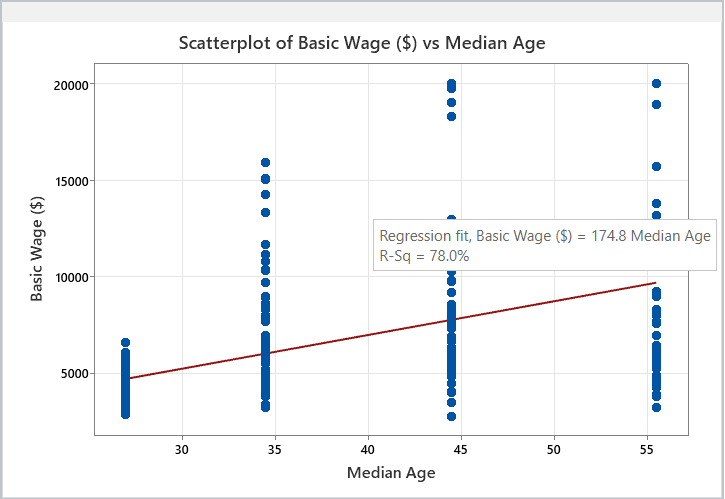
\includegraphics[width=0.75\linewidth]{MAI-Q1.png}
\caption{Scatter plot of Basic Wage vs Median Age with regression line (intercept = 0)}
\end{figure}

\textbf{Regression Equation from Minitab:}
\[
\widehat{\text{Basic Wage}} = 174.8 \text{ Median Age}
\]

%--------------------------------------------------------------------
\subsection{Question 1(b): Error Function and Derivative}

Since the intercept is fixed at zero, the regression model is
\[
\hat{y}_i = b x_i
\]

The mean squared error function is defined as:
\[
E(b)
= \frac{1}{232}
\Big[
(y_1 - b x_1)^2
+ (y_2 - b x_2)^2
+ \cdots
+ (y_{232} - b x_{232})^2
\Big]
\]

Differentiating $E(b)$ with respect to $b$ gives:
\[
E'(b)
= \frac{1}{232}
\Big[
2(y_1 - b x_1)(-x_1)
+ 2(y_2 - b x_2)(-x_2)
+ \cdots
+ 2(y_{232} - b x_{232})(-x_{232})
\Big]
\]

Simplifying $\left( \frac{2}{232} = \frac{1}{116} \right)$,
\[
E'(b)
= -\frac{1}{116}
\Big[
x_1(y_1 - b x_1)
+ x_2(y_2 - b x_2)
+ \cdots
+ x_{232}(y_{232} - b x_{232})
\Big]
\]

%--------------------------------------------------------------------
\subsection{Question 1(c): Gradient Descent Implementation}

\subsubsection{Question 1(c)(i): Python Code and Output}

\textbf{Python Code:}
\begin{verbatim}
import pandas as pd
import numpy as np
data = pd.read_excel("data/raw/Wages-2021-June.xlsx")
median_age = data["Median Age"].to_numpy(dtype=float)          # x
basic_wage = data["Basic Wage ($)"].to_numpy(dtype=float)      # y
num_points = len(median_age)                                   # n
slope_b = 0.0             # starting value of slope (b)
rate = 0.0001             # learning rate
epsilon = 0.00001         # stopping tolerance
diff = 1                  # difference between 2 consecutive b-values
max_iter = 150            # maximum number of iterations
iter = 1                  # iteration counter
error_E = lambda b: ((1 / num_points) *
                     np.sum((basic_wage - b * median_age) ** 2))
gradient_dE = lambda b: (-(2 / num_points) *
                         np.sum(median_age * (basic_wage - b * median_age)))
while diff > epsilon and iter < max_iter:
    new_slope_b = slope_b - rate * gradient_dE(slope_b)
    print("Iteration", iter, ": b-value is:",
          new_slope_b, "Error E(b) is:", error_E(new_slope_b))
    diff = abs(new_slope_b - slope_b)
    iter += 1
    slope_b = new_slope_b
print("Number of iterations is", iter - 1)
print("The local minimum occurs when b is", slope_b)
print("Minimum error is", error_E(slope_b))
\end{verbatim}
\textbf{Output:}
\begin{verbatim}
Number of iterations is 41
The local minimum occurs when b is 174.7967072224972
Minimum error is 13925464.984924644
\end{verbatim}

%--------------------------------------------------------------------
\subsubsection{Question 1(c)(ii): Final Regression Equation}

\[
\widehat{\text{Basic Wage}} = 174.8 \text{ Median Age}
\]

\textbf{Contextual Interpretation:}\\

The estimated slope is approximately $174.8$, indicating that each additional year
of Median Age increases the predicted Basic Wage by about \$174.80. This result is
consistent across both Minitab and the gradient descent method, with minor
differences arising from numerical approximation and the stopping criterion.

As the intercept is fixed at zero, the model assumes a direct proportional
relationship between Median Age and Basic Wage, which, while convenient, does not
fully reflect real-world wage behaviour.

%====================================================================
\section{Simple Linear Regression with Intercept}

\subsection{Model Definition}
The regression model is defined as:
\[
\hat{y}_i = a + b x_i
\]

where:
\begin{itemize}
    \item $\hat{y}_i =$ Predicted Basic Wage for the $i$-th observation
    \item $x_i =$ Median Age
\end{itemize}

%--------------------------------------------------------------------
\subsection{Question 2(a): Scatter Plot and Prediction (Minitab)}

\begin{figure}[H]
\centering
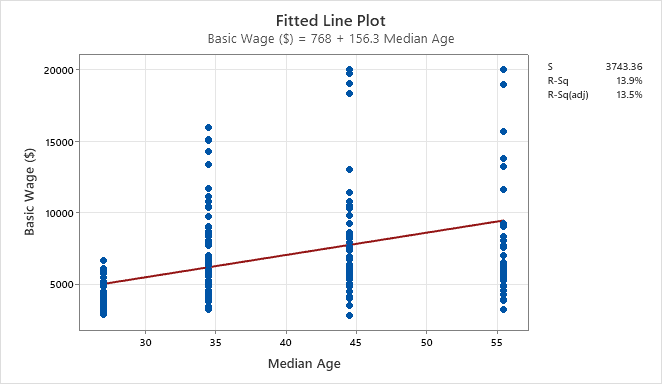
\includegraphics[width=0.75\linewidth]{MAI-Q2.png}
\caption{Scatter plot with regression line (intercept included)}
\end{figure}

\textbf{Regression Equation from Minitab:}
\[
\widehat{\text{Basic Wage}} = 768 + 156.3 \text{ Median Age}
\]

\textbf{Prediction Example:} \\
For Median Age = 30, \\
\[
\widehat{\text{Basic Wage}} = 768 + 156.3 \times 30
\]

\[
\widehat{\text{Basic Wage}} = 768 + 4689
\]

\[
\widehat{\text{Basic Wage}} = 5457
\]

Hence, when Median Age is 30 years, predicted Basic Wage is approximately \$5457.
%--------------------------------------------------------------------
%--------------------------------------------------------------------
\subsection{Question 2(b): Error Function and Partial Derivatives}

The mean squared error function is given by:
\[
E(a,b)
= \frac{1}{232}
\Big[
(y_1 - (a + b x_1))^2
+ (y_2 - (a + b x_2))^2
+ \cdots
+ (y_{232} - (a + b x_{232}))^2
\Big]
\]

\textbf{Partial derivative with respect to $a$:}
\[
\frac{\partial E}{\partial a}
= \frac{1}{232}
\Big[
2((a + b x_1) - y_1)
+ 2((a + b x_2) - y_2)
+ \cdots
+ 2((a + b x_{232}) - y_{232})
\Big]
\]

Simplifying $\left( \frac{2}{232} = \frac{1}{116} \right)$,
\[
\frac{\partial E}{\partial a}
= \frac{1}{116}
\Big[
(a + b x_1 - y_1)
+ (a + b x_2 - y_2)
+ \cdots
+ (a + b x_{232} - y_{232})
\Big]
\]

\textbf{Partial derivative with respect to $b$:}
\[
\frac{\partial E}{\partial b}
= \frac{1}{232}
\Big[
2((a + b x_1) - y_1)x_1
+ 2((a + b x_2) - y_2)x_2
+ \cdots
+ 2((a + b x_{232}) - y_{232})x_{232}
\Big]
\]

Simplifying $\left( \frac{2}{232} = \frac{1}{116} \right)$,
\[
\frac{\partial E}{\partial b}
= \frac{1}{116}
\Big[
(a + b x_1 - y_1)x_1
+ (a + b x_2 - y_2)x_2
+ \cdots
+ (a + b x_{232} - y_{232})x_{232}
\Big]
\]

%--------------------------------------------------------------------
\subsection{Question 2(c): Gradient Descent Solution}

\subsubsection{Question 2(c)(i): Python Code and Output}

\begin{verbatim}
import pandas as pd
import numpy as np
data = pd.read_excel("data/raw/Wages-2021-June.xlsx")
median_age = data["Median Age"].to_numpy(dtype=float)          # x
basic_wage = data["Basic Wage ($)"].to_numpy(dtype=float)      # y
num_points = len(median_age)                                   # n
mean_age = np.mean(median_age)
std_age = np.std(median_age)
median_age_scaled = (median_age - mean_age) / std_age
a_scaled = 0.0            # starting value of intercept (scaled model)
b_scaled = 0.0            # starting value of slope (scaled model)
learning_rate_a = 0.05    # learning rate for a_scaled
learning_rate_b = 0.05    # learning rate for b_scaled
epsilon = 1e-5            # stopping threshold
diff = 1                  # difference between consecutive iterates
max_iter = 1000           # maximum iterations
iter = 1                  # iteration counter
error_E = lambda a, b: ((1 / num_points) *
                        np.sum((a + b * median_age_scaled - basic_wage) ** 2))
grad_a = lambda a, b: ((2 / num_points) *
                       np.sum(a + b * median_age_scaled - basic_wage))
grad_b = lambda a, b: ((2 / num_points) *
                       np.sum((a + b * median_age_scaled - basic_wage) *
                              median_age_scaled))
while diff > epsilon and iter < max_iter:
    new_a_scaled = a_scaled - learning_rate_a * grad_a(a_scaled, b_scaled)
    new_b_scaled = b_scaled - learning_rate_b * grad_b(a_scaled, b_scaled)
    print("Iteration", iter, ": a_scaled =",
          new_a_scaled, ", b_scaled =", new_b_scaled,
          ", Error =", error_E(new_a_scaled, new_b_scaled))
    diff = max(abs(new_a_scaled - a_scaled), abs(new_b_scaled - b_scaled))
    iter += 1
    a_scaled, b_scaled = new_a_scaled, new_b_scaled
slope_b = b_scaled / std_age
intercept_a = a_scaled - (b_scaled * mean_age / std_age)
final_error = ((1 / num_points) *
               np.sum((basic_wage - (intercept_a + slope_b* median_age)) ** 2))
print("Number of iterations is", iter - 1)
print("The local minimum occurs when a is", intercept_a)
print("The local minimum occurs when b is", slope_b)
print("Minimum error is", final_error)
\end{verbatim}

\textbf{Output:}
\begin{verbatim}
Number of iterations is 173
The local minimum occurs when a is 767.5626075270866
The local minimum occurs when b is 156.2552942946782
Minimum error is 13891962.69841966
\end{verbatim}

%--------------------------------------------------------------------
\subsubsection{Question 2(c)(ii): Final Regression Equation}

\[
\widehat{\text{Basic Wage}} = 767.56 + 156.26 \text{ Median Age}
\]

\textbf{Contextual Interpretation:}

Using gradient descent, the estimated parameters were $a = 767.56$ and
$b = 156.26$ after 173 iterations. These values closely match the
coefficients obtained from Minitab, with minor differences arising from
numerical approximation and the stopping criterion. This close agreement
confirms that the gradient descent algorithm converged to the optimal
solution and validates the correctness of the implementation.

%--------------------------------------------------------------------
\subsection{Question 2(d): Convergence Discussion}

\begin{table}[H]
\centering
\scriptsize
\setlength{\tabcolsep}{3pt}
\caption{Experimental record for gradient descent parameter tuning in Model 2}
\label{tab:gd_experiment_record}
\begin{tabular}{|c|c|c|c|c|c|c|p{4.2cm}|}
\hline
\textbf{Trial} &
\textbf{Scaling} &
\textbf{Start $(a,b)$} &
$\boldsymbol{\text{rate}_a}$ &
$\boldsymbol{\text{rate}_b}$ &
$\boldsymbol{\epsilon}$ &
\textbf{Iter.} &
\textbf{Observation \& Justification} \\
\hline
1 & No & $(0,0)$ & 0.01 & 0.01 & $1\times10^{-5}$ &
$>$200{,}000 &
Extremely slow convergence due to poor numerical conditioning, indicating the need
for feature scaling. \\
\hline
2 & Yes & $(0,0)$ & 0.01 & 0.01 & $1\times10^{-5}$ &
815 &
Stable convergence observed, but iteration count remained high, suggesting that the
learning rates were conservative. \\
\hline
3 & Yes & $(0,0)$ & 0.05 & 0.05 & $1\times10^{-5}$ &
173 &
Smooth and efficient convergence with coefficients consistent with Minitab. Selected
as the final configuration. \\
\hline
4 & Yes & $(0,0)$ & 0.10 & 0.10 & $1\times10^{-5}$ &
85 &
Faster convergence was observed, but the selected learning rate of 0.05 was retained
as a more conservative final setting. \\
\hline
\end{tabular}
\end{table}

%====================================================================
\section{Multiple Linear Regression}

\subsection{Model Definition}
The multiple regression model is defined as:

\[
\hat{y}_i = a + b x_i + c w_i
\]

where:
\begin{itemize}
    \item $\hat{y}_i =$ Predicted Basic Wage for the $i$-th observation
    \item $x_i =$ Median Age
    \item $w_i =$ Average Overtime Hours Worked
\end{itemize}

%--------------------------------------------------------------------
\subsection{Question 3(a): Data Collection}

\textbf{Description of Variable $w$:} \\

In Model~3, an additional numerical predictor variable $w$ is introduced to represent
the total average overtime hours worked per month. This variable is inherently
quantitative and does not require encoding.

Average overtime hours capture labour intensity beyond normal contractual working
hours and are primarily driven by job demands and organisational workload rather than
age-related factors. This allows the effect of overtime on Basic Wage to be analysed
independently from the effect of Median Age.

In Singapore, overtime work is regulated under the Employment Act. According to the
Ministry of Manpower, overtime pay for eligible employees is calculated as
\[
\text{Overtime Pay}
= 1.5 \times \text{Hourly Basic Rate} \times \text{Overtime Hours}
\]
establishing a direct and proportional relationship between overtime hours and wage
compensation \cite{mom_overtime}. This supports the inclusion of average overtime hours
as a meaningful predictor of Basic Wage. Similar relationships between working time
and earnings have also been documented by the International Labour Organization and the
OECD \cite{ilo_overtime, oecd_hours}.

\textbf{Data Table Used:}

\begin{table}[H]
\centering
\small
\caption{Representative observations of Median Age, overtime hours, and Basic Wage}
\label{tab:overtime_wage_data}
\begin{tabular}{|c|c|c|}
\hline
\textbf{Median Age} &
\textbf{Avg. Overtime Hours (per month)} &
\textbf{Basic Wage (\$)} \\
\hline
27.0 & 10.25 & 2879 \\
27.0 & 10.25 & 3673 \\
34.5 & 11.79 & 4516 \\
34.5 & 11.79 & 4434 \\
34.5 & 11.79 & 5214 \\
44.5 & 13.48 & 4931 \\
44.5 & 13.48 & 5600 \\
44.5 & 13.48 & 7352 \\
55.5 & 12.69 & 5293 \\
55.5 & 12.69 & 6300 \\
\hline
\end{tabular}
\end{table}


\textbf{Data Collection Procedure:} \\
The Median Age and Basic Wage values were obtained directly from the
\textit{Wages 2021 June} dataset published by the Ministry of Manpower (MOM)
and were used as numerical variables without further transformation.

As the dataset does not include overtime information, data on working hours
was sourced from the \textit{Comprehensive Labour Force Survey 2021} to ensure
consistency in the reference year. Average overtime hours were derived by
identifying working hours beyond the standard contractual threshold defined
under the Employment Act and assigning representative monthly overtime values
based on the corresponding age-group working-hour distributions.

The resulting dataset combines observed wage and age data with overtime
values derived from official labour force statistics. These representative
observations are used for modelling purposes to examine the relationship
between Median Age, labour intensity, and Basic Wage, rather than to describe
individual workers.

%--------------------------------------------------------------------
\subsection{Question 3(b): Error Function and Partial Derivatives}

For Model~3, the regression model is defined as
\[
\hat{y}_i = a + b x_i + c w_i
\]
where $x_i$ represents the Median Age, $w_i$ represents the total average overtime
hours worked per month, and $\hat{y}_i$ denotes the predicted Basic Wage for the
$i$-th observation.

\subsubsection*{Error Function}

The mean squared error (MSE) function is given by
\[
E(a,b,c)
= \frac{1}{10}
\Big[
(y_1 - (a + b x_1 + c w_1))^2
+ (y_2 - (a + b x_2 + c w_2))^2
+ \cdots
+ (y_{10} - (a + b x_{10} + c w_{10}))^2
\Big]
\]

This function measures the average squared difference between the observed Basic
Wage values and the predicted values produced by the regression model.

\subsubsection*{Partial Derivatives}

\textbf{Partial derivative with respect to $a$:}
\[
\frac{\partial E}{\partial a}
= \frac{1}{10}
\Big[
2((a + b x_1 + c w_1) - y_1)
+ 2((a + b x_2 + c w_2) - y_2)
+ \cdots
+ 2((a + b x_{10} + c w_{10}) - y_{10})
\Big]
\]

Simplifying $\left( \frac{2}{10} = \frac{1}{5} \right)$,
\[
\frac{\partial E}{\partial a}
= \frac{1}{5}
\Big[
(a + b x_1 + c w_1 - y_1)
+ (a + b x_2 + c w_2 - y_2)
+ \cdots
+ (a + b x_{10} + c w_{10} - y_{10})
\Big]
\]

\textbf{Partial derivative with respect to $b$:}
\[
\begin{aligned}
\frac{\partial E}{\partial b}
&= \frac{2}{10}\sum_{i=1}^{10}
\big((a + b x_i + c w_i) - y_i\big)x_i \\
&= \frac{1}{5}\sum_{i=1}^{10}
(a + b x_i + c w_i - y_i)x_i
\end{aligned}
\]

\textbf{Partial derivative with respect to $c$:}
\[
\begin{aligned}
\frac{\partial E}{\partial c}
&= \frac{2}{10}\sum_{i=1}^{10}
\big((a + b x_i + c w_i) - y_i\big)w_i \\
&= \frac{1}{5}\sum_{i=1}^{10}
(a + b x_i + c w_i - y_i)w_i
\end{aligned}
\]

\subsubsection*{Mathematical Derivation}

Each partial derivative is obtained by differentiating the mean squared error
function with respect to one parameter at a time while holding the remaining
parameters constant. The derivative of each squared error term is computed using
the chain rule. Since the model is linear in $a$, $b$, and $c$, the derivatives of
$(a + b x_i + c w_i)$ with respect to $a$, $b$, and $c$ are $1$, $x_i$, and $w_i$
respectively. This results in the appearance of the factors $x_i$ and $w_i$ in the
partial derivatives with respect to $b$ and $c$.

\subsubsection*{Use in Gradient Descent}

The partial derivatives represent the gradients of the error function with respect
to the parameters $a$, $b$, and $c$. In the gradient descent algorithm, these
gradients are used to iteratively update the parameter values according to
\[
\theta_{\text{new}} = \theta_{\text{old}} - \alpha \frac{\partial E}{\partial \theta},
\quad \theta \in \{a, b, c\}
\]

where:
\begin{itemize}
    \item $\alpha =$ Learning Rate
\end{itemize}

At each iteration, the parameters are adjusted in the direction that reduces the
mean squared error. This process continues until the parameter updates become
sufficiently small, indicating convergence to values of $a$, $b$, and $c$ that
minimise the error function and define the regression model
\[
\hat{y} = a + b x + c w
\]

%--------------------------------------------------------------------
\subsection{Question 3(c): Coding, Results and Verification}

\textbf{Python Code:}
\begin{verbatim}
import pandas as pd
import numpy as np
data = pd.read_excel("data/processed/model3_data.xlsx")
median_age = data["Median Age"].to_numpy(dtype=float)
avg_overtime_hours = data["Average Overtime Hours per Month"].to_numpy(dtype=float)
basic_wage = data["Basic Wage ($)"].to_numpy(dtype=float)
num_points = len(median_age)
mean_age = np.mean(median_age)
std_age = np.std(median_age)
mean_overtime = np.mean(avg_overtime_hours)
std_overtime = np.std(avg_overtime_hours)
median_age_scaled = (median_age - mean_age) / std_age
overtime_scaled = (avg_overtime_hours - mean_overtime) / std_overtime
a_scaled = 0.0            # starting value of intercept (scaled model)
b_scaled = 0.0            # starting value of age coefficient (scaled model)
c_scaled = 0.0            # starting value of overtime coefficient (scaled model)
learning_rate_a = 0.05
learning_rate_b = 0.05
learning_rate_c = 0.05
epsilon = 0.001
diff = 1
max_iter = 1000
iter = 1
error_E = lambda a, b, c: (1 / num_points) * np.sum(
    (basic_wage - (a + b * median_age_scaled + c * overtime_scaled)) ** 2)
grad_a = lambda a, b, c: (2 / num_points) * np.sum(
    a + b * median_age_scaled + c * overtime_scaled - basic_wage)
grad_b = lambda a, b, c: (2 / num_points) * np.sum(
    (a + b * median_age_scaled + c * overtime_scaled - basic_wage)
    * median_age_scaled)
grad_c = lambda a, b, c: (2 / num_points) * np.sum(
    (a + b * median_age_scaled + c * overtime_scaled - basic_wage)
    * overtime_scaled)
while diff > epsilon and iter < max_iter:
    new_a_scaled = a_scaled - learning_rate_a * grad_a(a_scaled, b_scaled, c_scaled)
    new_b_scaled = b_scaled - learning_rate_b * grad_b(a_scaled, b_scaled, c_scaled)
    new_c_scaled = c_scaled - learning_rate_c * grad_c(a_scaled, b_scaled, c_scaled)
    print("Iteration", iter, ": a_scaled =", new_a_scaled,
        ", b_scaled =", new_b_scaled,
        ", c_scaled =", new_c_scaled,
        ", Error =", error_E(new_a_scaled, new_b_scaled, new_c_scaled))
    diff = max(abs(new_a_scaled - a_scaled), abs(new_b_scaled - b_scaled),
        abs(new_c_scaled - c_scaled))
    iter += 1
    a_scaled, b_scaled, c_scaled = new_a_scaled, new_b_scaled, new_c_scaled
coef_age = b_scaled / std_age
coef_overtime = c_scaled / std_overtime
intercept = (a_scaled - (b_scaled * mean_age / std_age)
            - (c_scaled * mean_overtime / std_overtime))
final_error = (1 / num_points) * np.sum(
    (basic_wage - (intercept + coef_age * median_age + coef_overtime *
    avg_overtime_hours)) ** 2)
print("Number of iterations is", iter - 1)
print("The local minimum occurs when a is", intercept)
print("The local minimum occurs when b is", coef_age)
print("The local minimum occurs when c is", coef_overtime)
print("Minimum error is", final_error)
\end{verbatim}
\textbf{Output:}
\begin{verbatim}
Number of iterations is 401
The local minimum occurs when a is -4273.116752825248
The local minimum occurs when b is 27.26077176350903
The local minimum occurs when c is 673.5503104554346
Minimum error is 438087.0501700889
\end{verbatim}

\textbf{Code Explanation:} \\
The dataset is loaded from an external Excel file, and the relevant variables are
extracted as numerical arrays. The predictor variables are standardised using their
means and standard deviations to improve numerical stability and convergence, as
Median Age and Overtime Hours are measured on different scales.

The mean squared error (MSE) is defined as the objective function to be minimised,
and its partial derivatives with respect to $a$, $b$, and $c$ are computed using the
\emph{prediction minus actual} formulation. These gradients are applied iteratively
to update the model parameters via gradient descent.

The algorithm terminates when the maximum change between successive parameter
updates falls below a specified tolerance. The estimated coefficients are then
transformed back to the original scale to obtain an interpretable regression
equation, and the final MSE is computed using the unscaled data to assess model fit.

\textbf{Regression Equation:}
\[
\widehat{\text{Basic Wage}} = -4273 + 27.3 \text{ Median Age} + 674 \text{ Avg. Overtime Hours per Month}
\]
\textbf{Contextual Interpretation:} \\
Holding other variables constant, an increase of one year in Median Age is associated
with an increase of approximately \$27.26 in Basic Wage, indicating a modest positive
relationship between age and wages.

In contrast, each additional hour of average overtime worked per month increases the
predicted Basic Wage by approximately \$673.55, reflecting a strong and direct link
between overtime work and wage compensation. This is consistent with statutory overtime
pay regulations in Singapore.

The intercept has no practical interpretation, as zero values for the predictors fall
outside the observed data range. Overall, the inclusion of overtime hours substantially
enhances the model by capturing labour intensity effects that are not explained by age
alone.

\textbf{Verification Method:} \\

To verify the gradient descent solution for Model~3, the same dataset was analysed
using Minitab's linear regression tool, with the estimated coefficients shown in
Figure~\ref{fig:model3_coefficients}. The coefficients obtained from both methods
are numerically consistent, with only minor differences due to rounding and
convergence tolerance, confirming that gradient descent successfully converged to
the optimal solution.

\begin{figure}[H]
\centering
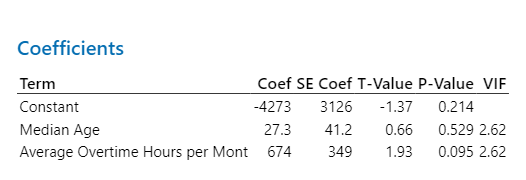
\includegraphics[width=0.75\linewidth]{MAI-Q3.png}
\caption{Minitab coefficient estimates for Model~3 used for verification}
\label{fig:model3_coefficients}
\end{figure}

%====================================================================
\bibliographystyle{unsrt}
\bibliography{references}

\end{document}
